% !TeX root = ../Thesis.tex

%*****************************************
\chapter{Related Work}\label{ch:relatedwork}
%*****************************************
\glsresetall % Resets all acronyms to not used

Steganography is often described as both the art and science of hiding information~\cite{bennettLinguisticSteganographySurvey2004}. As its forms are only limited by our creativity, an exhaustive discussion is not possible. Instead, we focus on some selected works. By progressing from simple to more sophisticated approaches, we ultimately answer the question: Why use \glspl{LLM} at all?

\section{Steganography without large language models}
\label{sec:steganographyWithoutLLMs}
As we implement an Android app to perform text-based steganography locally on smartphones, hardware resources are our strongest limitation. While \glspl{LLM} are a popular option to perform this kind of steganography~\cite{zieglerNeuralLinguisticSteganography2019}, running them is very resource-intensive. Therefore, we first consider some approaches without \glspl{LLM}.

\subsection{Mimicking}
\label{sec:mimicking}
Spammimic is a demonstration of text-based steganography without \glspl{LLM} from as early as 2001~\cite{spammimicSpammimic2000}. Secret messages are encoded into cover texts that look like spam e-mails. \cref{fig:spammimicSpamEmail} shows an example. This is done using context-free grammars and mimic functions~\cite{waynerMimicFunctions1992,bennettLinguisticSteganographySurvey2004}.

\begin{figure}
    \begin{wide}
        \centering
        \captionsetup{width=\linewidth}
        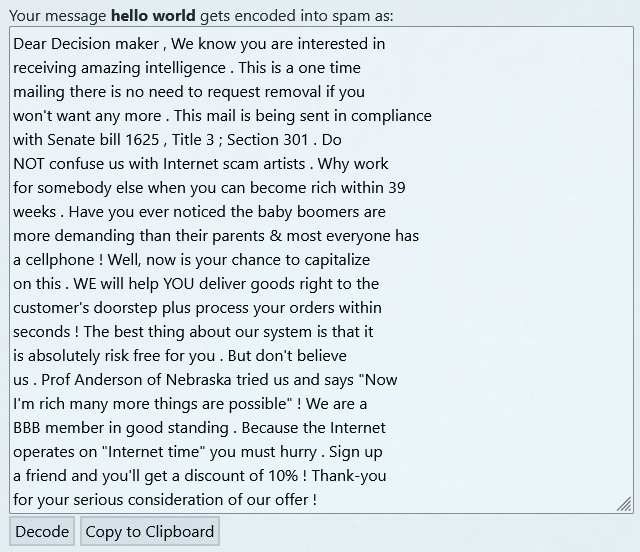
\includegraphics[width=0.5\linewidth]{spammimic_spam_email.png}
        \caption[Spammimic]{Steganography in spam e-mails with Spammimic~\cite{spammimicSpammimic2000}. Only the secret message "hello world" was user input.}
        \label{fig:spammimicSpamEmail}
    \end{wide}
\end{figure}

This approach already fulfills some of our requirements. It generates plausible cover texts for a given topic with minimal computing resources. The topic can be chosen by exchanging the grammar~\cite{spammimicSpammimic2000}. Generating spam e-mails is particularly beneficial as it lowers an attacker's expectation of cover text quality. It allows us to hide our communication amongst other e-mail traffic, obfuscating when a secret communication is happening. We may even send our cover texts to any number of recipients that includes the intended one, to obfuscate who is communicating with whom. Both would increase an attacker's costs significantly~\cite{bennettLinguisticSteganographySurvey2004,petitcolasInformationHidingSurvey1999}.

But there are several drawbacks. Users would have to handle different grammars for different chat conversations. Creating grammars requires expert knowledge. This can't be expected from the average user. In contrast, \glspl{LLM} can be influenced by natural language commands. This can be expected from any layman user. Furthermore, encoding efficiency is low. Any secret message longer than a few words generates cover texts of implausible length, even for a spam e-mail.

\subsection{Substitution}
\label{sec:substitution}
When \gls{SMS} was prevalent, its character limits led users to abbreviate common terms (e.g. "u" for "you"). As shown in ~\cite{shirali-shahrezaTextSteganographySMS2007}, this can be leveraged to perform steganography. We define a dictionary of terms and their abbreviations and let the user write a chat message without any abbreviations. By either substituting terms with their abbreviations or not, we encode 1s and 0s.

This approach again fulfills some of our requirements. It uses minimal computing resources and gives the user great control over cover text quality. Semantically meaningful conversations are guaranteed as terms and their abbreviations are synonymous. A customizable dictionary is already built into the keyboards of most smartphones, so it is easily accessible for the average user.

But there still are several drawbacks. As many terms don't have an abbreviation in practice, encoding efficiency is low. This is aggravated when abbreviations are used for entire sentences instead of individual words (e.g. "ily" instead of "i luv u" for "i love you"). Abbreviations can be undesired for readability or even inappropriate in formal communication. Other substitution approaches (e.g. substituting synonym words) solve these issues only partially.

\subsection{Further considerations}
\label{sec:furtherConsiderations}
In the previous sections of this chapter, we discussed several approaches for text-based steganography without \glspl{LLM}. In particular, we focussed on the extent to which each approach fulfilled our central requirement - creating a believable chat conversation from cover texts. In this section, we take a look at some more text-based steganography approaches, still without involving \glspl{LLM}. But the focus is now on some more refined requirements, stemming from more specific use cases. Lastly, we take a look at an example of what not to do.

\subsubsection{Localization}
\label{sec:localization}
The overall goal of our implementation can be stated as follows: Use text-based steganography in chat messages to protect against attackers. While multiple aspects of this definition can and will be refined over the course of this thesis, we now discuss one aspect that is largely omitted otherwise: Localization. Our standard assumption is that both users and attackers are English-speaking. This may be fine for academic purposes, but in practice a lot of the potential users of our implementation are in countries where English is not an official language. This is especially relevant for protection from political persecution under authoritarian regimes.

An example implementation of location-specific steganography is Nahoft~\cite{united4iranNahoft2021,united4iranU4iadminNahoft2025}. This is an Android app designed to protect people in Iran protesting against their government. It performs text-based steganography by creating cover texts consisting of random Persian words, the official language of Iran. If English was used in this situation, it would only attract unwanted attention from the authorities.

Characteristics specific to languages with non-Latin scripts can be leveraged for steganography. Examples for such languages are Arabic~\cite{shirali-shahrezaNewApproachPersian2006,hamzahLinguisticSteganographyFramework2021,thabitComparativeAnalysisArabic2021}, Chinese~\cite{luoTextSteganographyHigh2017} and Hindi~\cite{allaEvolutionHindiText2009}. The scripts of these languages provide a rich variety of symbols and variations, exceeding what the Latin script has to offer, allowing e.g. multiple equivalent shapes for the same expression~\cite{shirali-shahrezaNewApproachPersian2006,hamzahLinguisticSteganographyFramework2021,thabitComparativeAnalysisArabic2021}. Furthermore, relationships between languages should be considered. Steganography approaches leveraging language-specific characteristics can sometimes be transferred to related languages~\cite{allaEvolutionHindiText2009}.

The challenge of localization can partially be solved with our implementation. As~\cref{ch:design} will explain in detail, one goal of our implementation is that the \gls{LLM} can be swapped out easily. While this doesn't enable us to leverage language specifics like changing character shapes, it enables us to choose a \gls{LLM} that was trained on any natural language desired. If we are able to generate semantically meaningful cover texts in any language, further localization might not be necessary. We could use our implementation in any geo-political conflict, deliberately speaking (or not speaking) the language of the attacker. But verifying this is unfortunately out of scope for this thesis, as the author doesn't speak any languages with non-Latin scripts.

\subsubsection{A negative example}
\label{sec:aNegativeExample}
Lastly, we take a look at an example of what not to do, so we can avoid it in our implementation. We recall that steganography violates Kerckhoffs' principle~\cite{andersonLimitsSteganography1998}, as the security of a steganographic system partially relies on the attacker not knowing the system - or that it is being used in the first place.

An approach for text-based steganography in e-mails is shown in~\cite{malikHighCapacityText2017}. Similar to our implementation, it uses Huffman compression to convert a secret message from string to binary. But instead of generating a cover text with \glspl{LLM}, an edit-based approach is chosen by taking the cover text from user input. Information is encoded by colour coding the cover text, with colours being selected from a user-defined colour table. \cref{fig:colourCoding} shows the example given in~\cite{malikHighCapacityText2017}. As~\cite{malikHighCapacityText2017} proposes, this approach is suitable for personal messages containing congratulations, poems, etc. Users may try to obfuscate the steganography as they have full control over cover text quality and the colour table, e.g. by choosing black, dark grey, light grey and white as colours.

\begin{figure}
    \begin{wide}
        \centering
        \captionsetup{width=\linewidth}
        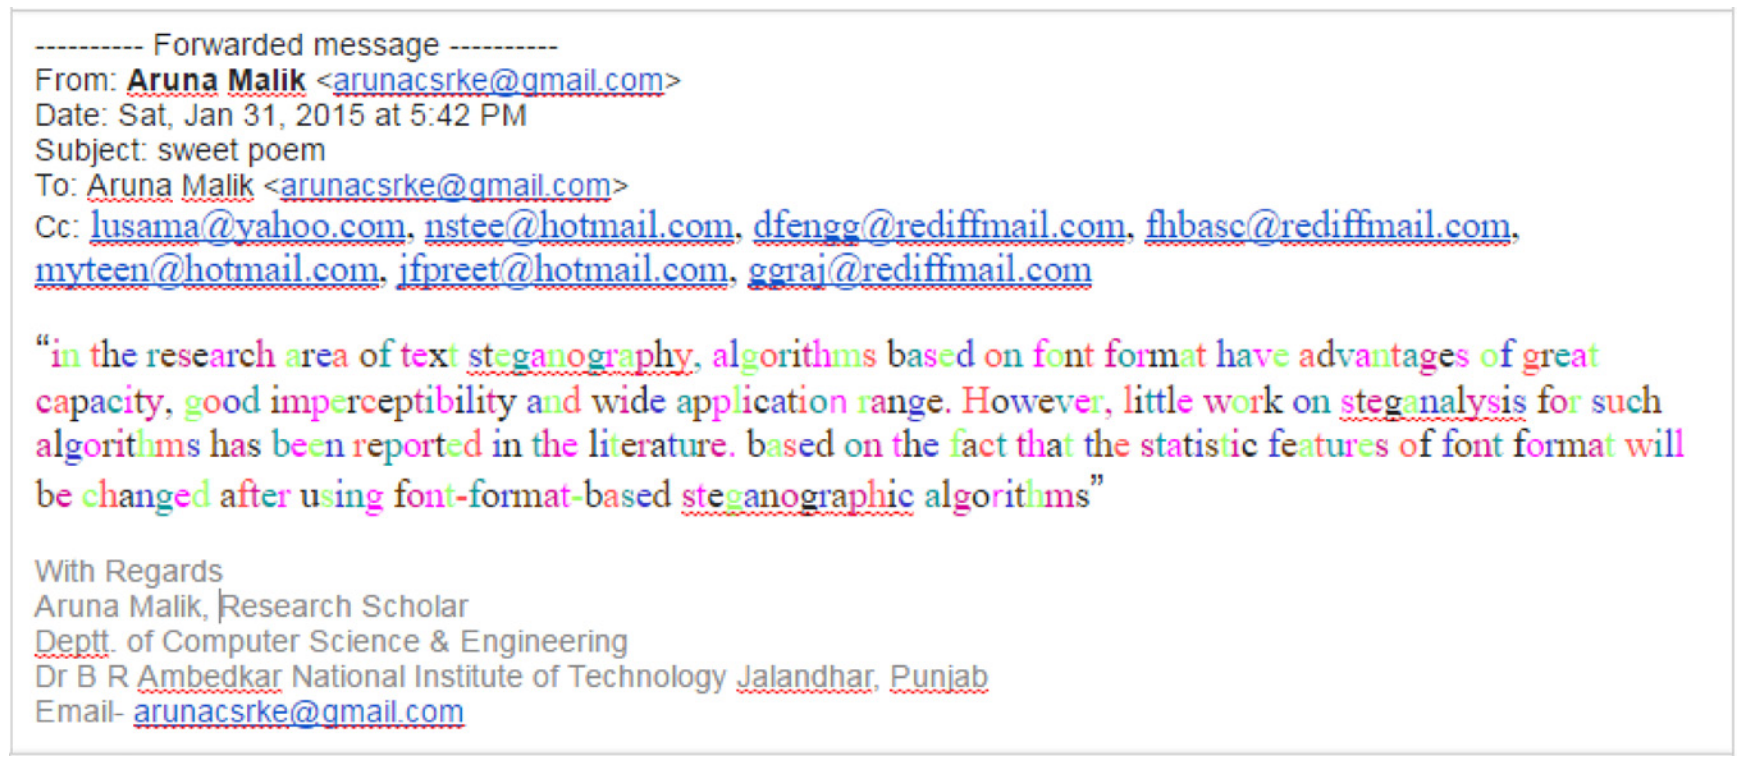
\includegraphics[width=0.75\linewidth]{colour_coding.png}
        \caption[Colour coding]{Steganography via colour coding~\cite{malikHighCapacityText2017}.}
        \label{fig:colourCoding}
    \end{wide}
\end{figure}

However, this doesn't outweigh the disadvantages. The colour table has to be exchanged between sender and receiver, which is difficult as it is not natural language. This approach also is not robust when using non-digital communication channels, as the colour coding is lost if the cover text is spoken during a phone call or printed out in black and white. The proposed use case is very narrow, as an attacker should become suspicious if this is used in any other setting. More generally, the colour coding introduces an unnatural communication pattern that might make it obvious to an attacker that a secret communication is happening. This breaks the additional layer of security that is supposed to be introduced by steganography. We can transfer this to our implementation by avoiding e.g. uncommon use of abbreviations or emojis in the generated chat conversations. Furthermore, we should also avoid introducing unnatural restrictions, e.g. assuming that chat messages are being sent with strictly alternating roles of sender and receiver. \cref{ch:implementation} will show that this is only partially possible in our implementation.

\section{Steganography with large language models}
\label{sec:steganographyWithLLMs}
In the last section, we investigated how text-based steganography can be performed without involving \glspl{LLM}. Historical approaches were mostly edit-based, as the ability to generate coherent text was limited~\cite{zieglerNeuralLinguisticSteganography2019}. This changed with the introduction of the Transformer architecture~\cite{vaswaniAttentionAllYou2023} in 2017, which laid the foundation for the popular \gls{AI} chatbots we know today.

In this section, we first consider high-level approaches that only involve prompting the \gls{LLM} to perform steganography. Then, we consider low-level approaches that manipulate the token generation of the \gls{LLM}. This finally leads us to the paper this thesis is based on~\cite{zieglerNeuralLinguisticSteganography2019}.

\subsection{High-level: Prompting}
\label{sec:highLevelPrompting}
With state-of-the-art \glspl{LLM} reaching hundreds of billions of parameters, they are able to comprehend long contexts and perform advanced logic only by being prompted~\cite{hossainLLMProSAnalyzingLarge2025}. \gls{AI} chatbots like ChatGPT help users solve problems in all fields of science and engineering~\cite{schmidgallAgentLaboratoryUsing2025}, from solving physics equations~\cite{songLLMFeynmanLeveragingLarge2025,panQuantumManybodyPhysics2025} to writing and debugging code~\cite{leeGitHubRecentBugs2024,leeUnifiedDebuggingApproach2024,tianDebugBenchEvaluatingDebugging2024,shiCodeCorrectnessClosing2024}. This suggests that we might be able to instruct a \gls{LLM} to behave like a steganographic system, i.e. to generate a cover text that encodes a secret message.

As demonstrated in~\cite{steinebachNaturalLanguageSteganography2024,wuPromptingSteganographyNew2024} with ChatGPT, it is possible to perform steganography by prompting \glspl{LLM}. We will focus on~\cite{steinebachNaturalLanguageSteganography2024}, as its approach is simpler and the relevant advantages and disadvantages are similar to~\cite{wuPromptingSteganographyNew2024}.

A possible approach to perform steganography via prompting works as follows (simplified)~\cite{steinebachNaturalLanguageSteganography2024}: Define two disjoint sets of words, A and B. Instruct the LLM to generate a text that contains words from A and B matching a certain pattern (e.g. BABBABABA). Interpret any occurence of a word from set A as a 0 bit, any of a word from set B as a 1 bit. Use this logic to define a pattern matching the desired bit sequence, thereby encoding a secret message in the generated cover text.

This approach is attractive because it only requires high-level access to the \gls{LLM}. The user doesn't need to understand technical details like tokenization or tensors to influence the behaviour of the \gls{LLM}. The topic of the cover text can be controlled via the words in sets A and B, which themselves can be generated with a single prompt. Efficiency can be improved by increasing the number of sets to choose from~\cite{steinebachNaturalLanguageSteganography2024}, thereby encoding more bits of information within every selected word. It is also relatively efficient in computing resources, as the \gls{LLM} is only needed for encoding, while decoding can be performed deterministically given a cover text and the word sets. Quality of cover texts can too be controlled easily. If a previously generated cover text is not satisfactory, only reprompting is needed. This suggests that generating a conversation from cover texts is plausible too.

Although this approach may be able to fulfill the central requirement for our implementation, it conflicts with almost every other goal and requirement we set ourselves. As even the largest \glspl{LLM} struggle with reliability~\cite{vendrowLargeLanguageModel2025}, they still make encoding errors with the careful prompt engineering demonstrated in~\cite{steinebachNaturalLanguageSteganography2024,wuPromptingSteganographyNew2024}, thereby corrupting the secret message. For any smaller \gls{LLM} that is feasible to run locally on a smartphone, this will be aggravated. This would make the core functionality of our implementation dependent on cloud-based service providers. These providers would be able to tie the secret messages to our identities. As already detailed in \cref{sec:makingAVirtueOutOfNecessity}, this increases attack surface immensely: We would expose ourselves to both outside attackers and the commercial interests of the service provider. Furthermore, this approach is not to be desired as availability would not be ensured. While large commercial service providers generally have good uptime records, an implementation relying on them would require a constant internet connection and access to the provider's domain. Recalling the use case of protection from authoritarian regimes mentioned in~\cref{sec:localization}, the latter is a non-trivial assumption, as such regimes often block undesirable domains country-wide~\cite{wongSocialMediaMay2016,michaelsonJournalistsMore11002025}. Lastly, even though this is a generation-based approach, encoding efficiency is not very high. While it can be controlled via the number of word sets as described above, the examples given in~\cite{steinebachNaturalLanguageSteganography2024} show that most words in the cover text don't encode any information. This suggests that the simplicity of this approach is not worth largely giving up privacy and immensely increasing the attack surface.

\subsection{Low-level: Manipulating token generation}
\label{sec:lowLevelManipulatingTokenGeneration}
The last section reinforced several further requirements for our implementation: It should be local-first and work offline to introduce as little third party dependencies as possible. We cannot rely on commercial providers for access to the most powerful \glspl{LLM}, but have to run a smaller \gls{LLM} locally. This restricts the possible complexity of prompts significantly (see~\cref{ch:design} for details), leading us to consider a more low-level approach to influence the behaviour of the \gls{LLM}.

A possible approach is demonstrated in Stegasuras~\cite{zieglerNeuralLinguisticSteganography2019,zieglerHarvardnlpNeuralSteganography2025,zieglerStegasuras2025}, which serves as the foundation for this thesis. It implements steganography by manipulating the token generation of the \gls{LLM}. This requires low-level access to tokenizers and tensors, which none of the previous approaches considered. Arithmetic, Huffman and Bins encoding algorithms are implemented using GPT-2 and PyTorch (see~\cref{ch:design} and~\cref{ch:implementation} for corresponding details of our implementation).

This approach is promising several strengths we haven't seen before. By gaining low-level access to the \gls{LLM}, we can implement a complex encoding logic. This wouldn't be possible via prompting due to the limited selection of \glspl{LLM} imposed by the restrictions of mobile devices. It allows us to reach a significantly higher encoding efficiency than previous approaches~\cite{zieglerNeuralLinguisticSteganography2019}.

Fundamentally, it works as follows: A secret message is first converted from string to binary. A cover text is then generated by selecting tokens from the predictions of the \gls{LLM} for a given context. This selection is based on a logic that processes the secret message bits, thereby encoding information within each selected token~\cite{zieglerNeuralLinguisticSteganography2019}. The logic by which the tokens are selected can be exchanged, i.e. the three algorithms mentioned above can be seen as one generic algorithm with a variable sampling method.

Arithmetic coding is used not only for steganography, but also for compressing the secret message during its binary conversion~\cite{zieglerNeuralLinguisticSteganography2019}. For long strings with known probability distribution this compression is optimal, i.e. it compresses them to their entropy~\cite{rissanenArithmeticCoding1979}. In practice, it is often more efficient than Huffman compression~\cite{zieglerNeuralLinguisticSteganography2019} (see~\cref{ch:implementation} for further discussion). This further increases encoding efficiency and lowers the barrier for small \glspl{LLM} to generate believable cover texts.

While this suggests that steganography with local \glspl{LLM} might be feasible on smartphones, the implementation demonstrated in~\cite{zieglerStegasuras2025} is not without issues. Most notably, being published in 2019, it is not state-of-the-art anymore. Significant gains in cover text quality are to be expected by just swapping out the \gls{LLM}~\cite{wuGenerativeTextSteganography2024}.

Furthermore, there is an edge case that is not covered in any of the implemented algorithms. While encoding, the \gls{LLM} will generate cover text tokens until all bits of the secret message are processed. As it stands, this would mean that token generation ends abruptly while the cover text might be in the middle of a sentence. Such a cover text would look highly suspicious to an attacker, rendering this approach unusable for creating believable chat conversations. While the code provided at~\cite{zieglerHarvardnlpNeuralSteganography2025} already contains a flag to finish the last sentence of the cover text by greedy sampling, it is not used. Simply setting this flag from \lstinline|false| to \lstinline|true| doesn't solve the issue though, since the decoding functions don't consider it. This creates noise when recovering a secret message, as tokens from greedy sampling don't contain any information.

While this issue is important to factor in when judging cover text quality and therefore real world use, it is ignored in the evaluation of Stegasuras~\cite{zieglerNeuralLinguisticSteganography2019}: Participants were presented four sentences of text, the first three taken from news articles and used as context, the last one generated by the \gls{LLM}. They were then asked to judge if the fourth sentence is a plausible continuation of the first three. Any output of the \gls{LLM} longer than one sentence was cut off~\cite{zieglerNeuralLinguisticSteganography2019}, thereby corrupting the cover text and rendering the secret message unrecoverable. A more sensible solution would have been to let the \gls{LLM} finish its last sentence and to clean up the noise in decoding.

Improving the implementation by solving this challenge is the first contribution this thesis makes (see \cref{ch:implementation} for our solution). Beyond that, the value of this thesis is created in multiple ways. The implementation will be extended to generate a believable chat conversation from cover texts. This is done by leveraging the context that is passed to the \gls{LLM} (see \cref{ch:implementation}). We will show that it is feasible to run all of this locally on a smartphone by the example of the Android platform. We provide our own implementation using a state-of-the-art framework (see \cref{ch:design}). We will show how to handle irregularities in human communication (e.g. sending plain texts in-between cover texts, using emojis or allowing multiple consecutive messages from the same sender). Lastly, we will increase control over cover text quality further by not just passing a context to the \gls{LLM}, but also by implementing a system prompt for easy low-level access. This way, we are able to solve the real-world use case of protecting people from attackers with steganography.
